\documentclass{article}
\usepackage[utf8]{inputenc}
\usepackage{graphicx}
\usepackage{makecell}
\usepackage{color}
\usepackage{amsmath}
\usepackage{wrapfig}
\usepackage{tikz}
\usetikzlibrary{arrows,shapes,chains,automata}

\title{Computer Architecture Homework 4}
\date{Spring 2023, March}

\begin{document}

\maketitle
\setlength{\headsep}{-30pt}
\setlength{\footskip}{100pt}
\section{Boolean Algebra and Logic Gates}
\noindent For the circuit shown below:\par
\begin{figure}[htbp]
	\centering
	\includegraphics[width=1.0\linewidth]{/Users/songyulu/Desktop/CS110_hw4/q1.png}
	\label{fig:1}
\end{figure}
\noindent a. Write the Boolean Expression of the circuit and simplify it step by step (as simple as possible).{\color{red} (10 pts)}

\newpage
\noindent b. Write the Truth Table of the simplified Boolean Expression.{\color{red} (10 pts)}
\begin{table}[h!]
\centering
\setlength{\tabcolsep}{5mm}
\begin{tabular}{|c|c|c|c|}
\hline
A & B & C & Output \\ \hline
1 & 1 & 1 &  \\ \hline
1 & 1 & 0 &  \\ \hline
1 & 0 & 1 &  \\ \hline
1 & 0 & 0 &  \\ \hline
0 & 1 & 1 &  \\ \hline
0 & 1 & 0 &  \\ \hline
0 & 0 & 1 &  \\ \hline
0 & 0 & 0 &  \\ \hline
\end{tabular}
\end{table}
~\\
~\\
~\\

\noindent c. Create a circuit of Boolean Expression Y = A + B using only NAND gates.{\color{red} (10 pts)}


\newpage

\section{FSM}

\noindent a.
\begin{figure}[htbp]
	\centering
	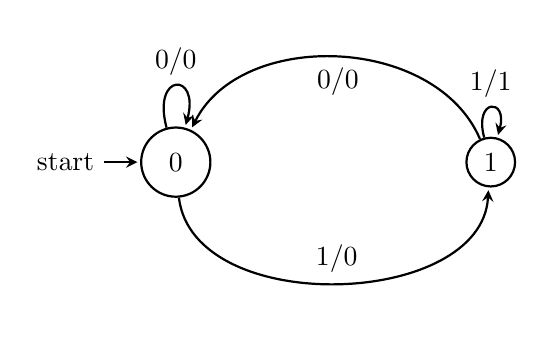
\begin{tikzpicture}[->,>=stealth,shorten >=1pt,auto,node distance=4cm,
		thick,base node/.style={circle,draw,minimum size=16pt}, real node/.style={double,circle,draw,minimum size=35pt}]
		
		\node[shape=circle,draw=black,initial,state](0){0};
		\node[shape=circle,draw=black](1)[right of=0 ]{1};
		
		\path[]
		(0) edge [loop above]node {0/0} (0)	
		(1) edge [loop above]node {1/1} (1)	
		(0) edge [bend right=85]node {1/0} (1)
		(1) edge [bend right=65]node {0/0} (0);
		
	\end{tikzpicture}
\end{figure}\\
\noindent (1) {\color{red} (5 pts)}Start with the initial state, the FSM outputs a 1 if it detects the pattern (bitstring) :\\
\noindent (2) {\color{red} (5 pts)}What would it output for the input bitstring "011001110"?
~\\
~\\
~\\

\noindent b. Draw a FSM that outputs 1 when it receives two or more successive '0'. Complete the following graph.{\color{red} (20 pts)}
\begin{figure}[htbp]
	\centering
	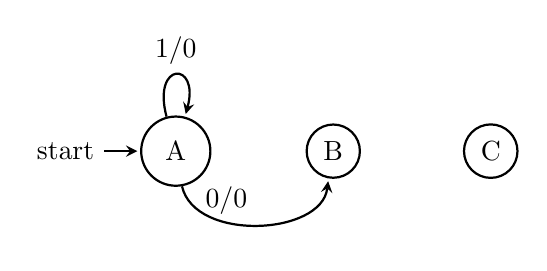
\begin{tikzpicture}[->,>=stealth,shorten >=1pt,auto,node distance=2cm,
		thick,base node/.style={circle,draw,minimum size=16pt}, real node/.style={double,circle,draw,minimum size=35pt}]
		
		\node[shape=circle,draw=black,initial,state](00){A};
		\node[shape=circle,draw=black](01)[right of=00 ]{B};
		\node[shape=circle,draw=black](10)[right of=01 ]{C};
		
		\path[]
		(00) edge [loop above]node {1/0} (00)		
		(00) edge [bend right=80]node {0/0} (01);
		
	\end{tikzpicture}
\end{figure}\\
~\\

\noindent c. Fill out the remainder of the table for the FSM in (b).{\color{red} (10 pts)}
\begin{table}[h!]
\centering
\setlength{\tabcolsep}{5mm}
\begin{tabular}{|l|l|l|l|l|l|l|l|l|l|}
\hline
Input      & \multicolumn{1}{c|}{-} & 1 & 0 & 0 & 1 & 0 & 1 & 0 & 0 \\ \hline
Next State & A                      &   &   &   &   &   &   &   &   \\ \hline
Output     & -                      &   &   &   &   &   &   &   &   \\ \hline
\end{tabular}
\end{table}

\newpage

\section{SDS}

In the following circuit, NOT gates have a delay of 1ns, AND gates have a delay of 4ns, NAND gates have a delay of 6ns, OR gates have a delay of 3ns. The registers have a clk-to-q delay of 4ns and setup times of 6ns. Assume the inputs comes from registers and output is connected to a register. All the delays refer to propagation delay.\par
\begin{figure}[htbp]
	\centering
	\includegraphics[width=1.0\linewidth]{/Users/songyulu/Desktop/CS110_hw4/q3.png}
	\label{fig:1}
\end{figure}
\noindent a. What is the minimum acceptable clock cycle time for this circuit? What clock frequency does it correspond to?  (please include enough explanation){\color{red} (20 pts)}
~\\
~\\
~\\
~\\
~\\
~\\
~\\
~\\
~\\
~\\
~\\
~\\
~\\
~\\

\noindent b. What is the maximum allowable hold time for the registers that allows this circuit run correctly? (please include enough explanation){\color{red} (10 pts)}

\end{document}
